\documentclass[lang=cn,12pt,chinesefont=founder,toc=twocol]{elegantbook}

\title{数理统计笔记}
\author{肖程哲}
\date{\today}
%\version{}
%\bioinfo{自定义}{信息}

\extrainfo{苟日新,日日新,又日新}

\setcounter{tocdepth}{3}

\logo{logo.png}
\cover{cover.jpg}

\usepackage{array, fdsymbol, float, bbm,tabularx,booktabs,multirow,bm,subcaption}
\usetikzlibrary{decorations.pathreplacing,decorations.pathmorphing,arrows.meta,patterns}
\usepackage[below]{placeins}
\usepackage[free-standing-units]{siunitx}
% \usepackage{tikz}
% \usetikzlibrary{external}
% \tikzexternalize[prefix=figures/]
% \newcommand{\inputtikz}[1]{%
%   \tikzsetnextfilename{#1}%
%   \input{#1.tikz}%
% }

\newcommand{\iidsim}{\widesim[2.33]{\mathrm{i.i.d.}}}	% independent and identically distributed
\newcommand{\indep}{\perp\!\!\!\perp}		% independent
\newcommand{\1}{\mathbbm{1}}				% indicator
\renewcommand{\P}{\mathbb{P}}				% probability
%\renewcommand{\Pr}{\operatorname{P}}		% probability
\newcommand{\as}{\mathrm{a.s.}}				% almost surely
\newcommand{\E}{\mathbb{E}}					% expectation
\newcommand{\Var}{\operatorname{Var}}		% variance
\newcommand{\Cov}{\operatorname{Cov}}		% covariance
\newcommand{\MSE}{\operatorname{MSE}}		% mean square error
\newcommand{\mean}[1]{\overline{#1}}
\newcommand{\abs}[1]{\left\lvert#1\right\rvert}		% absolute value
\newcommand{\norm}[1]{\left\lVert#1\right\rVert}
\newcommand{\rank}[1]{\operatorname{rank}\left(#1\right)}
\newcommand{\tr}[1]{\operatorname{tr}\left(#1\right)}		% trace
\newcommand{\diag}[1]{\operatorname{diag}\!\left(#1\right)}			% diagonal
\newcommand{\vspan}[1]{\operatorname{span}\left(#1\right)}	% vector span
\newcommand{\proj}[2]{\operatorname{proj}_{#2}#1}			% projection
\newcommand{\inprod}[2]{\left\langle #1, #2 \right\rangle}	% inner product
\newcommand{\R}{\mathbb{R}}					% real
\renewcommand{\d}{\mathrm{d}}				% differential
\newcommand{\pd}{\partial}					% partial differential
\newcommand{\p}[3][]{\frac{\pd^{#1}#2}{\pd{#3}^{#1}}}	% partial derivative
\newcommand{\e}{\varepsilon}
\newcommand{\st}{\mathrm{s.t.}\ }			% subject to, so that
\newcommand{\argmin}{\operatornamewithlimits{arg\,min}}
\newcommand{\argmax}{\operatornamewithlimits{arg\,max}}
\newcommand{\N}{\mathcal{N}}				% normal, not natural numbers XD
\newcommand{\vs}{\; \operatorname{vs}\;}
\newcommand{\red}{\color[HTML]{FE0000}}

\setlist[description]{
	labelindent = 4em,
	labelwidth = 7em,
	leftmargin = 11em,
	labelsep = 0em,
	parsep = 0.75em,
	topsep = 0.75em,
}

%\includeonly{src/3.Point_Estimation}
\begin{document}

\maketitle
\frontmatter
\tableofcontents

\mainmatter
\chapter{导论: 从数据中学习}\label{ch:intro}

统计学的主要研究内容是如何收集和处理\emph{随机数据}。数据的随机性一方面来源于自然物理机制中不可避免的随机性;一方面来源于不能被控制(或者不关心)的其他因素。收集数据时,应尽量使其具有代表性(常通过分层抽样实现)。从数据中获取信息,并借此\emph{解释}和\emph{预测}数据的过程称为\emph{推断}(inference)。统计推断基于概率模型,对两个基本问题:\emph{估计}(estimation)与\emph{检验}(testing)进行回答。为了有效地使用数据进行统计推断,需要给定某些准则去评判不同统计推断方法的优劣。

\section{统计模型}\label{sec:inference}

\begin{definition}[样本]
      在实验中获取的观测值$\mathbf{x}=(x_1, \cdots ,x_n)$视为某个概率空间$(\Omega,\mathscr{F},\P)$上的随机元$X$的\underline{实现}(realization)。概率测度$\P$称为总体,观测值或其对应的随机元称为\textbf{样本}(sample),这组观测值的数目$n$称为\textbf{样本容量}(sample size)。
\end{definition}

\begin{definition}[总体]
      假设样本来源于各分量$X_i$独立同分布的随机向量,其分布$P(\bullet):=\P\{X_i \in \bullet\}$称为\textbf{总体}(population)。
\end{definition}

在统计学中可以认为总体$P$包含我们想知道的一切信息,然而(至少部分)是未知的。我们希望用样本$\mathbf{x}$推断总体$P$的性质。

\begin{definition}[参数]
      在总体中固定但未知的常数称为\textbf{参数}, 记为$\theta$. 参数所有可能的取值构成\textbf{参数空间}, 记为$\Theta$, 可以是有限维或者无限维。
\end{definition}
\begin{remark}
      参数的函数同样固定且未知,故也视为参数. 
\end{remark}

\begin{definition}[统计模型]
      \textbf{统计模型}(statistical model)是样本$\mathbf{X}$对应的所有可能的总体$P$的集合。在同一统计模型中,不同的总体通过参数区分,所以将模型记为:
      \[ \mathcal{P}=\{ P_{\theta}:\theta \in \Theta \} \]
\end{definition}

统计模型代表关于数据产生机制的先验(prior)知识。

\begin{definition}[可识别]
      若模型$\mathcal{P}=\{ P_{\theta}:\theta \in \Theta \}$满足:
      \[ P_{\theta_1} \neq P_{\theta_2}, \forall \theta_1 \neq \theta_2 \]
      则称模型$\mathcal{P}$\textbf{可识别}(identifiable)
\end{definition}

\begin{definition}
      若$\Theta$有限维的,则称模型$\mathcal{P}$为\textbf{参数族}(parametric family);若参数空间$\Theta$是无限维的,则称为\textbf{非参数族}。
\end{definition}

我们常常只关心参数$\Theta$的某些分量的函数$\gamma=g(\theta)$,剩下的碍事且无用的部分称为\textbf{冗余参数}(nuisance parameter)。

\section{统计量}

\begin{definition}[统计量]
      给定样本$X_1,\cdots ,X_n \overset{\text{i.i.d.}}{\sim} P$,其中$P \in \mathcal{P}$是未知的总体. 若$ T:(\mathcal{X}_n,\mathscr{F}^n_\mathcal{X})\to (\mathcal{T} ,\mathscr{F}_\mathcal{T})$是已知的(不依赖$P$的)可测函数,则称$T(\mathbf{X})=T(X_1,\cdots ,X_n)$为\textbf{统计量}(statistic)。
\end{definition}

\begin{definition}
      统计量的分布称为它的\textbf{抽样分布}(sampling distribution), 含有总体 (样本分布) 的一部分信息.
\end{definition}

统计量函数, 不依赖未知总体, 给出了一种数据约简(reduction). 

\begin{problemset}[错题记录]
      \item (茆5.5.10)设$x_1,\dotsc,x_n$是来自正态分布$N(\mu,\sigma^2)$的样本,在$\mu$已知时给出$\sigma^2$的一个充分统计量
  \end{problemset}

\chapter{描述性统计}

\section{单变量样本}

设$x = \{x_1,\dots,x_n\}$ 是单变量样本 $X_1,X_2,\cdots,X_n$ 的一个实现。这些随机变量独立同分布。

一个分布通常有两个重要的数值特征:位置(location)和散度(dispersion)。位置通常由均值和中位数描述。若分布是对称的,则两者等价;若分布右偏(左偏),则均值大于(小于)中位数。对于一个未知的分布,通常使用样本均值和样本中位数描述其位置。

\begin{definition}[样本均值]\label{def:sample mean}
    将样本 $X_1,X_2,\cdots,X_n$ 的一个统计量 
    \[ \overline{X} = \frac1n\sum_{i=1}^{n}X_{i}. \]
    称为\textbf{样本均值}(sample mean)。
\end{definition}

\begin{definition}[样本均值]\label{def:sample median}
    将样本 $X_1,X_2,\cdots,X_n$ 的一个统计量 
    \[ M = \operatorname{med}(x) = \begin{cases}
        x_{(\frac{n+1}{2})} & n \text{为奇数} \\
        \frac{x_{(\frac{n}{2})} + x_{(\frac{n}{2}+1)}}{2} & n \text{为偶数}
    \end{cases} \]
    称为\textbf{样本中位数}(sample median)。其中顺序统计量$x_{(1)}\leq\dots\leq x_{(n)}$由$x_1,\dots,x_n$排列得到。
\end{definition}

分布的散度则对应着方差(或标准差)和四分位数(interquartile range, IQR)。


\begin{description}
      \item [样本均值](sample mean)
            \[ \bar{x} = \frac1n\sum_{i=1}^{n}x_{i}. \]
      \item [样本方差](sample variance)
            \[ s^{2} = \frac{1}{n-1}\sum_{i=1}^{n}(x_{i}-\bar{x})^{2}. \]
            由此可得\textbf{样本标准差}(sample standard deviation) $s = \sqrt{s^2}$.
      \item [样本中位数](sample median)
            \[ M = \operatorname{med}(x) = \begin{cases}
                        \quad x_{(k)},                  & n = 2k-1 \\
                        \frac{1}{2}(x_{(k)}+x_{(k+1)}), & n = 2k
                  \end{cases} \]
            
      \item [四分位数](quartile)
            \[ Q_{1} = \operatorname{med}(x\cap(-\infty,M)), \qquad
                  Q_{3} = \operatorname{med}(x\cap(M,+\infty)). \]
      \item [四分位距](inter quartile range)
            \[ \mathit{IQR} = Q_{3} - Q_{1}. \]
      \item [极差](range)
            \[ x_{(n)}-x_{(1)} = \max(x)-\min(x) = \max_{1\leq i,i' \leq n}\{x_{i}-x_{i'}\}. \]
\end{description}

\begin{definition}[经验分布函数]
      样本 $X_1,X_2,\cdots,X_n$ 的\textbf{经验分布函数}为:
      \[ F_n(x) = \frac1n\sum_{i=1}^n \1{X_i \le x}  \]
\end{definition}

\subsection{直方图}

\subsection{箱线图}

\begin{definition}
      \textbf{五数概括法}(five-number summary): 以$x_{(1)},Q_{1},M,Q_{3},x_{(n)}$总结$x$, 可用\textbf{箱线图}(boxplot)表示.
\end{definition}

\subsection{QQ图}



\section{相关性}
\chapter{点估计}

\begin{introduction}[考试重点]
    \item 矩估计和极大似然估计
    \item 点估计的其他评价方法
    \item UMVUE
    \item (弱)相合和强相合
    \item Fisher信息量和有效估计
    \item 贝叶斯估计
\end{introduction}

\begin{definition}[点估计]
    用于估计参数$\gamma = g(\theta)$的统计量$T(x)$称为\textbf{估计量}(estimator), 记为$\hat{\gamma} = T(X)$. 估计式是随机变量, 若给定统计模型, 则其分布由参数$\theta$决定, 将观测数值代入估计式后得到的值称为\textbf{估计值}.
\end{definition}

将数据代入估计式得到的估计值并不是真实的参数值,若使用新的样本,很可能会得到不同的估计值。

\section{点估计的评价方法}

\subsection{无偏性}

\begin{definition}[无偏估计]
    估计式的\textbf{偏差}(standard error)定义为其抽样分布的均值与实际参数的偏差, 即:
    \[ E(\hat{\theta})-\theta \]
    若其为零, 则称此估计为参数$\theta$的\textbf{无偏估计}
\end{definition}

\begin{example}[方差的无偏估计]
    \begin{align*}
        s^2    & = \frac1{n-1} \sum_{i=0}^n (X_i-\bar{X})^2=\frac1{n-1} [\sum_{i=0}^n X_i^2 - n\bar{X}^2]                                                                         \\
               & =\frac1{n-1} [\sum_{i=0}^n X_i^2 - \frac1n  (\sum_{i=0}^n X_i)^2] = \frac1{n-1} [\sum_{i=0}^n X_i^2 - \frac1n  (\sum_{i=0}^n X_i^2 + \sum_{i \neq j}^n X_i X_j)] \\
               & = \frac1n  \sum_{i=0}^n X_i^2 - \frac1{n(n-1)} \sum_{i \neq j}^n X_i X_j                                                                                         \\
        E(s^2) & = \frac1n  \sum_{i=0}^n E(X_i^2) - \frac1{n(n-1)} \sum_{i \neq j}^n E(X_i X_j) = \mu_2-m_1^2=\sigma^2
    \end{align*}
\end{example}

\begin{definition}[渐进无偏估计]
    若样本量趋于无穷时,估计式的偏差为零,即:
    \[ \lim_{n \to \infty}E(\hat\theta_n)=\theta \]
    则称此估计为参数$\theta$的\textbf{渐近无偏估计}
\end{definition}

\begin{example}[样本方差的渐进无偏性]
    对于样本方差$s_n^2 = \frac1n  \sum_{i=0}^n (X_i-\bar{X})^2$,其期望为$E(s_n^2) = \frac{n-1}n \sigma^2$。当样本量趋于无穷时,有$E(s^{*2})\to\sigma^2$。故$s^{*2}$为$\sigma^2$的渐近无偏估计。
\end{example}

无偏性\underline{不具有不变性},即若$\hat{\theta}$是$\theta$的无偏估计,一般而言,其函数$g(\hat{\theta})$不是$g(\theta)$的无偏估计,除非$g(\theta)$是$\theta$的线性函数。譬如,$s^2$是$\sigma^2$的无偏估计,但$s$不是$\sigma$的无偏估计。

\begin{example}
    设总体为$N(\mu,\sigma^2), x_1, \cdots, x_n$是样本,考察$s$是否是$\sigma$的无偏估计。$Y=\frac{(n-1)s^2}{\sigma^2} \sim \chi^2(n-1)$,其密度函数为
    \[ p(y)=\frac1{2^{\frac{n-1}2} \Gamma(\frac{n-1}2)} y^{\frac{n-1}2-1}\ee^{-\frac{y}2}, \quad y>0 \]
    从而
    \begin{align*}
        E(Y^{1/2}) & =\int_0^{+\infty} y^{1/2} p(y)\d y = \frac1{2^{\frac{n-1}{2}} \Gamma(\frac{n-1}2)} \int_0^{\infty} y^{\frac{n}{2}-1} \ee^{-\frac{y}{2}} \dd y   \\
                   & =\frac{2^{\frac{n}{2}} \Gamma(\frac{n}{2})}{2^{\frac{n-1}{2}} \Gamma(\frac{n-1}{2})}=\sqrt{2} \frac{\Gamma(\frac{n}{2})}{\Gamma(\frac{n-1}{2})}
    \end{align*}
    由此,我们有
    \[E(s)=\frac{\sigma}{\sqrt{n-1}} E(Y^{1/2})=\sqrt{\frac2{n-1}} \cdot \frac{\Gamma(n/2)}{\Gamma((n-1)/2)} \cdot \sigma \]
    这说明$s$不是$\sigma$的无偏估计。
\end{example}

当参数存在无偏估计时,我们称该参数是\textbf{可估}的,否则称它是不可估的。

\subsection{有效性}

% \begin{definition}[标准误差]
%     估计式的\textbf{标准误差}(standard error)定义为其抽样分布的标准差, 即:
%     \[ \sqrt{\operatorname{Var}_{\theta}(\hat{\theta})} \]
% \end{definition}

参数的无偏估计可以有很多,如何在无偏估计中进行选择?直观的想法是希望该估计围绕参数真值的波动越小越好,波动大小可以用方差来衡量,因此人们常用无偏估计的方差的大小作为度量无偏估计优劣的标准,这就是有效性.

\begin{definition}[有效性]
    设$\hat\theta_1,\hat\theta_2$是$\theta$的两个\underline{无偏估计},如果对任意的$\theta\in\Theta$有
    \[ \Var(\hat\theta_1) \le \Var(\hat\theta_2),  \]
    且至少有一个$\theta\in\Theta$使得上述不等号严格成立,则称$\hat\theta_1$比$\hat\theta_2$\textbf{有效}。
\end{definition}

\subsection{均方误差}
无偏性是估计的一个优良性质,对无偏估计我们还可以通过其方差进行有效性比较.然而不能由此认为:有偏估计一定是不好的估计.

在有些场合,有偏估计比无偏估计更优,这就涉及如何对有偏估计进行评价.一般而言,在样本量一定时,评价一个点估计的好坏使用的度最指标总是点估计值与参数真值8的距离的函数,最常用的函数是距离的平方.由于具有随机性,可以对该函数求期望,

\begin{definition}\label{def:MSE}
    估计式与参数的平方的期望称为\textbf{均方误差}
    \[ \text{MSE}(\hat\theta) = E(\hat\theta-\theta)^2 \]
\end{definition}

注意到
\begin{align*}
    \text{MSE}(\hat\theta) & = [ E(\hat\theta - E\hat\theta) + (E\hat\theta - \theta)^2 ]                                                     \\
                           & = E (\hat\theta - E\hat\theta)^2 + (E\hat\theta - \theta)^2 + 2E[(\hat\theta - E\hat\theta)(E\hat\theta-\theta)] \\
                           & = \Var(\hat\theta) + (E\hat\theta - \theta)^2
\end{align*}

因此,均方误差由点估计的方差与偏差的平方两部分组成。如果$\hat\theta$是$\theta$的无偏估计,则$\text{MSE}(\hat\theta)=\Var(\hat\theta)$,此时用均方误差评价点估计与用方差是一样的;当$\hat\theta$不是$\theta$的无偏估计时,就要看其均方误差$\text{MSE}(\hat\theta)$,即不仅要看其方差大小,还要看其偏差大小。

\begin{definition}[一致最小均方误差估计]\label{def:minimum_MSE_estimation}
    在一个估计类中,若其中的一个估计式$\hat{\theta}$对估计类中任意一个估计式$\tilde{\theta}$,在参数空间$\Theta$上满足
    \[ \text{MSE}_{\theta}(\hat\theta) \le \text{MSE}_{\theta}(\tilde\theta) ,\quad \forall \theta \in \Theta  \]
    则称此估计式为该估计类中$\theta$的\textbf{一致最小均方误差估计}。
\end{definition}

\begin{example}
    对均匀总体$U(0,\theta)$,考虑$\theta$的形如$\hat\theta_\alpha = \alpha\cdot x_{(n)}$的估计,其均方误差为
    \begin{align*}
        \text{MSE}(\hat\theta_\alpha) & = \Var(\alpha\cdot x_{(n)}) + (\alpha Ex_{(n)} - \theta) ^2                                 \\
                                      & = \alpha^2\Var(x_{(n)}) + \left( \alpha\frac n{n+1}\theta - \theta \right)^2                \\
                                      & = \alpha^2 \frac n{(n+1)^2(n+2)} + \left( \frac{n\cdot \alpha}{n+1} - 1 \right)^2\theta^2 .
    \end{align*}
    用求导的方法不难求出当$\alpha_0=(n+2)/(n+1)$时上述均方误差达到最小,此时$\text{MSE}\left(\frac{n+2}{n+1}x_{(n)}\right)=\frac{\theta^2}{(n+1)^2}$。$\hat\theta_0=\frac{n+2}{n+1}x_{(n)}$虽是$\theta$的有偏估计,但对于无偏估计$\hat\theta=\frac{n+1}{n}x_{(n)}$而言,其均方误差$\text{MSE}(\hat\theta_0)=\frac{\theta^2}{(n+1)^2}<\frac{\theta^2}{n(n+2)}=\text{MSE}(\hat\theta)$。所以在均方误差的标准下,有偏估计$\hat\theta_0$优于无偏估计$\hat\theta$。并且$\hat\theta_0$为形如$\alpha\cdot x_{(n)}$的估计类中$\theta$的一致最小均方误差估计。
\end{example}

若不对估计加以限制(即考虑所有可能的估计),则一致最小均方误差估计是不存在的,从而没有意义。事实上,若$\hat\theta$是$\theta$的所有估计中的一致最小均方误差估计,取定任一个$\theta_0 \in Theta$,令$\tilde\theta=\theta_0$, 则$\text{MSE}_{\theta_0}(\tilde\theta)=0$,于是要求$\hat\theta_0$也有$\text{MSE}_{\theta_0}(\hat\theta)=0$,由$\theta_0$的任意性,这意味着$\text{MSE}_{\theta}$处处为$0$,这显然是做不到的。

\subsection{相合性}

\begin{definition}[相合]
    若当样本容量$n\to\infty$时, 有
    \[ \hat{\gamma} \xrightarrow{\P} \gamma, \quad \forall \theta\in\Theta. \]
    则称$\hat{\gamma}$是\textbf{相合的/一致的}(consistent), 如果上式中$\xrightarrow{\P}$可以增强为$\xrightarrow{\as}$, 则称$\hat{\gamma}$是\textbf{强相合的}.
\end{definition}
\begin{remark}
    由于参数是常数,所以依概率收敛与依分布收敛等价。
\end{remark}

若把依赖于样本量$n$的估计量$\hat\theta_n$看作一个随机变量序列,相合性就是$\hat\theta_n$依概率收敛于$\theta$,所以证明估计的相合性可应用依概率收敛的性质及各种大数定律。反过来也一样,由Kolmogorov 强大数定律可知,若样本独立同分布,且总体的期望存在的话,则\emph{样本均值必定为其期望的强相合估计}。同时,如果样本的方差存在的话,则\emph{样本方差必定为其方差的强相合估计}。

\begin{example}
    设$x_1,\cdots,x_n$是来自正态总体$N(\mu,\sigma^2)$的样本,则由辛钦大数定律及依概率收敛的性质知:
    \begin{itemize}
        \item$\bar x$是$\mu$的相合估计;
        \item$s^{*2}$是$\sigma^2$的相合估计;
        \item$s^2$也是$\sigma^2$的相合估计。
    \end{itemize}
    由此可见参数的相合估计不止一个。
\end{example}

\begin{theorem}[相合性定理]
    设$\hat\theta_n=\hat\theta_n(x_1,\cdots,x_n)$是$\theta$的一个估计量, 若
    \[ \lim_{n \to \infty} E(\hat\theta_n)=\theta, \quad \lim_{n \to \infty} \operatorname{Var}(\hat\theta_n)=0 \]
    则$\hat\theta_n$是$\theta$的相合估计,
\end{theorem}
\begin{proof}
    由切比雪夫不等式有
    \[ P(|\hat\theta_n - E(\hat\theta_n)| \ge \e/2) \le \frac{4}{\e^2} \operatorname{Var}(\hat\theta_n), \quad \forall  \e>0\]
    另一方面,由$\lim_{n \to \infty} E(\hat\theta_n)=\theta$可知
    \[ \exists N , \forall n>N \st |E(\hat\theta_n)-\theta| < \e/2\]
    注意到如果$|\hat\theta_n-E(\hat\theta_n)|<\e/2$,就有
    \[ |\hat\theta_n - \theta| \le |\hat\theta_n - E(\hat\theta_n)|+|E(\hat\theta_n) - \theta| < \e\]
    故
    \[ \{|\hat\theta_n - E(\hat\theta_n)| < \e/2\} \subset \{ | \hat\theta_n - \theta | < \e \} \]
    等价地
    \[ \{ |\hat\theta_n - E(\hat\theta_n)| \ge  \e/2 \} \supset \{|\hat\theta_n - \theta| \ge \e \}\]
    由此即有
    \[ P(|\hat\theta_n - \theta| \ge \e) \le P(|\hat\theta_n - E(\hat\theta_n)| \ge \e/2) \le \frac{4}{\e^2} \operatorname{Var}(\hat\theta_n) \to 0 \]
\end{proof}

\begin{theorem}[相合估计的连续映射]
    若$\hat{\theta}_{n1},\cdots,\hat{\theta}_{nk}$分别是$\theta_1,\cdots,\theta_k$的相合估计,$\eta=g(\theta_1,\cdots,\theta_k)$是$\theta_1,\cdots,\theta_k$的连续函数,则$\bar{\eta}_n=g(\hat{\theta}_{n1},\cdots,\hat{\theta}_{nk})$是$\eta$的相合估计。
\end{theorem}
\begin{proof}
    由函数$g$的连续性,对$\forall \e>0$,存在$\exists \delta>0$,当满足$|\hat{\theta}_j-\theta_j|<\delta,j=1,\cdots,k$时,有
    \[ |g(\hat{\theta}_1, \cdots, \hat{\theta}_{k})-g(\theta_1, \cdots, \theta_{k})|<\e \]
    即
    \[ \bigcap_{j=1}^k \{|\hat{\theta}_{n j}-\theta_j| < \delta\} \subset \{ | \hat\eta_n - \eta | < \e \} \]
    又由$\hat{\theta}_{n1},\cdots,\hat{\theta}_{nk}$的相合性得
    \[ \forall v>0 ,\exists N \in N_+, \forall n>N \st P(|\hat{\theta}_{n j}-\theta_{j}| \ge \delta)<v/k, \quad j=1, \cdots, k\]
    从而有
    \begin{align*}
        P\left(\left|\hat{\eta}_n -\eta\right|<\e\right) & >
        P\left(\bigcap_{i=1}^k\{|\hat{\theta}_{n j} - \theta_j|<\delta\}\right)                                                              \\
                                                         & = 1-P\left(\bigcup_{j=1}^k\{ | \hat{\theta}_{n j}-\theta_j | \ge \delta\}\right) \\
                                                         & \ge 1-\sum_{j=1}^k P(|\hat{\theta}_{n j}-\theta_j| \ge \delta)                  \\
                                                         & >1 - k \cdot v/k = 1-v
    \end{align*}
    由$v$的任意性,定理得证。
\end{proof}

\subsection{渐近正态性}

\begin{definition}[渐近正态性]
    对于参数$\tau(\theta)$的相合估计$T_n$,若存在趋于$0$的非负常数序列$\sigma_n(\theta)$,使得
    \[ \frac{T_n - \tau(\theta)}{\sigma_n(\theta)} \xrightarrow{d} N(0,1) \]
    则称$T_n$是\textbf{渐近正态}的,服从渐近正态分布$N(\tau(\theta),\sigma_n(\theta)^2)$,记为$T_n \sim AN(\tau(\theta),\sigma_n(\theta)^2)$,$\sigma_n(\theta)^2$为$T_n$的\textbf{渐近方差}或$T_n$的极限分布的方差。
\end{definition}
\begin{remark}
    $\sigma_n(\theta)$表示着估计量$T_n$依概率收敛于$\tau(\theta)$的速度。由中央极限定理可看出,通常为$\frac1{\sqrt{n} }$量级。
\end{remark}

\begin{example}
    设总体为泊松分布$P(\lambda)$,以样本均值为其参数估计,即
    \[ \hat\lambda_n=\bar{x_n} \]
    由中心极限定理,$\frac{\hat\lambda_n-\lambda}{\sqrt{\lambda/n}}$依分布收敛于$N(0,1)$,因此,$\hat\lambda_n$是渐近正态的,
\end{example}

\section{点估计的方法}

\subsection{矩估计}

\begin{definition}[总体矩与样本矩]
    若$X_1,\cdots ,X_n \overset{\text{i.i.d.}}{\sim} P_{\theta}$,记$k$阶\textbf{总体矩}为:
    \[ \mu_k(\theta) = \E_{\theta}[X_i^k] ,\quad k \in \mathbb{N} \]
    记$k$阶\textbf{样本矩}为:
    \[ \hat\mu_k=\frac1n \sum_{i=1}^n X_i^k ,\quad k \in \mathbb{N} \]
\end{definition}

% \begin{definition}[矩法估计量]
%     参数$\gamma = g(\theta)$的\textbf{矩{\color{lightgray}(法)}估计量}(method of moments estimator)定义为
%     \[ \hat{\gamma}^{\mathrm{MoM}} = g(\hat{\theta}^{\mathrm{MoM}}) , \]
%     其中$\hat{\theta}^{\mathrm{MoM}}$对选定的$k$满足
%     \[ \mu_{k}(\hat{\theta}^{\mathrm{MoM}}) = \hat{\mu}_{k} . \]
% \end{definition}

矩方法的步骤:
\begin{enumerate}
    \item 将低阶矩通过参数表达,一般阶数与待估参数个数相同$\bf\mu=f(\bf\theta)$;
    \item 找出上一步骤的反函数,通过矩表达参数$\bf\theta=f^{-1}(\bf\mu)$;
    \item 将样本矩代入,得到参数的估计式$\hat{\theta}=f^{-1}(\hat{\bf\mu})$
    \item 将参数的矩估计式代入函数$g(\bf\theta)$,得到参数的函数$\eta = g(\theta)$的矩估计。
\end{enumerate}
\begin{remark}
    对于参数的函数的估计,矩估计和极大似然估计都是将对参数的估计代入。但极大似然估计的做法是根据其不变性;而矩估计是源于定义,不保证与函数的矩估计相同。
\end{remark}

\begin{example}[泊松分布的矩估计]\label{moment_estimate_Poisson}
    设$X_1, \cdots ,X_n \overset{\text{i.i.d.}}{\sim} P(\lambda)$,则其一阶矩$\mu_1=\lambda$,所以$\lambda=\mu_1$,其矩估计为:
    \[ \hat{\lambda} = \hat{\mu_1} = \overline{X} \]
\end{example}

\begin{example}
    设$X_1,\dots,X_n$是独立同分布的连续型随机变量, 具有p.d.f.
    \[ f_{\lambda,a}(x) = \lambda\mathrm{e}^{-\lambda(x-a)}\1_{[x>a]}, \quad x\in\R, \]
    其中$\lambda > 0$和$a \in \R$未知(\emph{注}: 相应的统计模型是带有\emph{位置}(location)参数和\emph{速率}(rate)参数的指数分布). 易见$X_i \stackrel{d}{=} a + Y/\lambda$, 其中$Y \sim \mathrm{Exponential}(1)$. 利用$\E[Y]=1$和$\E[Y^2] = 2$, 可以得到
    \[ \mu_1(\lambda,a) = a + 1/\lambda, \quad\&\quad
        \mu_2(\lambda,a) = a^2 + 2a/\lambda + 2/\lambda^2 . \]
    方程
    \[ \mu_{k}(\hat{\lambda}^{\mathrm{MoM}},\hat{a}^{\mathrm{MoM}}) = \hat{\mu}_{k}, \quad k = 1,2 \]
    的解
    \[ \hat{\lambda}^{\mathrm{MoM}} = 1\Big/\sqrt{\hat{\mu}_2-\hat{\mu}_1^2}, \quad\&\quad
        \hat{a}^{\mathrm{MoM}} = \hat{\mu}_1-\sqrt{\hat{\mu}_2-\hat{\mu}_1^2} \]
    即为$(\lambda,a)$的一种矩估计.
\end{example}

\begin{proposition}[矩估计的无偏性]\label{prop:MME_unbiased}
    $k$阶样本矩是关于总体分布$k$阶矩的无偏估计。
\end{proposition}
\begin{proof}
    \[ E(\hat\mu_k)=\frac1n \sum_{i=1}^n E(X_i^k)=\mu_k \]
\end{proof}

\begin{remark}
    对$k\ge 2$,样本$k$阶中心矩不是总体$k$阶中心矩的无偏估计。
\end{remark}

\begin{example}
    对于2阶中心矩(即方差)有:
    
\end{example}

\begin{proposition}[矩估计的相合性]
    矩估计都是相合估计
\end{proposition}
\begin{proof}
    由命题\ref{prop:MME_unbiased}可知, 矩估计的
\end{proof}

\subsection{极大然似估计}

极大然似估计的基本思想:对于参数空间中的每一个参数,计算在此参数下,观测数据的发生概率,选取最大概率对应的参数。

\begin{definition}[然似函数]
    设随机变量$X_1,\cdots ,X_n$的联合密度函数(或质量函数)为$f(x_1,\cdots ,x_n|\theta)$。对于某一组观测数据$x_1^* ,\cdots ,x_n^*$,其\textbf{然似函数}(likelihood function)为:
    \[ \mathfrak{L}(\theta) = f(x_1^* ,\cdots ,x_n^*|\theta) \]
    对\textbf{数然似函数}(log likelihood function)为$l(\theta)=\log\mathfrak{L}(\theta)$
\end{definition}
\begin{remark}
    联合密度质量函数代表概率,但联合密度函数不是,代表概率所占比例;两者都是变量$x$的函数。然似函数是关于参数$\theta$的函数,不是概率,对整个参数空间的积分未必等于一。
\end{remark}

\begin{definition}[极大然似估计]
    可使然似函数取最大值的参数被称为\textbf{极大然似估计},即
    \[ \hat{\theta}=\max_{\theta \in \Theta}\mathfrak{L}(\theta) \]
\end{definition}
\begin{remark}
    由于对数函数单调递增,最大化然似函数等价于最大化对数然似函数。
\end{remark}

若样本来源变量独立同分布,即$f(x_1,\cdots ,x_n|\theta)=\prod_{i=1}^nf(x_i|\theta)$,则其然似函数和对数然似函数分布可写为:
\[ \mathfrak{l}(\theta) = \prod_{i=1}^nf(x_i^*|\theta), \quad l(\theta) = \sum_{i=1}^n \log f(x_i^*|\theta) \]

\begin{proposition}[极大然似估计的不变性]
    设$\hat{\theta}$是参数$\theta$的极大然似估计,那么对于参数$\theta$的任意函数$\gamma = g(\theta)$,其极大然似估计$\hat{\gamma}=g(\hat{\theta})$
\end{proposition}
\begin{proof}
    %TODO
\end{proof}

\subsection{贝叶斯估计}

贝叶斯估计的基本观点是:任一未知量$\theta$都可看作随机变量,可用概率分布$\pi(\theta)$描述,称为\textbf{先验分布};在获得样本之后,总体分布、样本与先验分布通过贝叶斯公式结合起来得到关于未知量$\theta$的后验分布$\pi(\theta | \bf{X})$。任何关于$\theta$的统计推断都基于$\theta$的后验分布进行。利用后验分布$\pi(\theta|\bf{X})$估计$\theta$有三种常用的方法:
\begin{itemize}
    \item 使用后验分布的密度函数最大值点作为$\theta$的点估计的最大后验估计;
    \item 使用后验分布的中位数作为$\theta$的点估计的后验中位数估计;
    \item 使用后验分布的均值作为$\theta$的点估计的后验期望估计.
\end{itemize}
用得最多的是后验期望估计, 它一般也简称为贝叶斯估计, 记为的$\hat{\theta}_B$。

获取后验分布的步骤:
\begin{enumerate}
    \item 根据总体信息与样本信息确定模型$p(\bf{X} | \theta)$,根据先验信息确定参数$\theta$的先验分布$\pi(\theta)$
    \item 综合总体信息、样本信息和先验信息得到样本$\bf{X}$和参数$\theta$的联合分布
          \[h(\bf{X}, \theta)=p(\bf{X}|\theta) \pi(\theta)\]
    \item 为求后验分布$\pi(\theta|\bf{X})=\frac{h(\bf{X}, \theta)}{m(\bf{X})}$,先求$X$的边际概率函数:
          \[ m(\bf{X})=\int_{\bf{\theta}} h(\bf{X}, \theta) \mathrm{d} \theta=\int_{\bf{\theta}} p(\bf{X}| \theta) \pi(\theta) \mathrm{d} \theta \]
    \item 得到后验分布
          \[ \pi(\theta | \bf{X})=\frac{h(\bf{X}, \theta)}{m(\bf{X})}=\frac{p(\bf{X} | \theta) \pi(\theta)}{\int_{\bf{\theta}} p(\bf{X} | \theta) \pi(\theta) \mathrm{d} \theta} \]
\end{enumerate}

\begin{definition}[共扼先验分布]
    设$\theta$是总体参数,$\pi(\theta)$是其先验分布, 若对任意的样本观测值得到的后验分布$\pi(\theta|\bf{X})$与$\pi(\theta)$属于同一个分布族, 则称该分布族是$\theta$的\textbf{共扼先验分布(族)}。
\end{definition}

\begin{example}
    设某事件$A$在一次试验中发生的概率为$\theta$,为估计$\theta$,对试验进行了$n$次独立观测,其中事件$A$发生了$X$次,显然$X | \theta \sim b(n, \theta)$,即
    \[P(X=x | \theta)=\binom{n}{x} \theta^{x}(1-\theta)^{n-x}, \quad x=0,1, \cdots, n\]
    假若我们在试验前对事件$A$没有什么了解,从对其发生的概率也没有任何信息。在这种场合,贝叶斯本人建议采用“同等无知”的原则,使用区间$(0,1)$上的均匀分布$U(0,1)$作为$\theta$的先验分布。贝叶斯的这个建议被后人称为贝叶斯假设。
\end{example}
\begin{solution}
    先写出$X$和$\theta$的联合分布
    \[ h(x, \theta)=\binom{n}{x} \theta^x (1-\theta)^{n-x}, \quad x=0,1, \cdots, n, \quad 0<\theta<1\]
    然后求$X$的边际分布
    \[ m(x)=\binom{n}{x} \int_0^1 \theta^x (1-\theta)^{n - x} \d \theta=\binom{n}{x} \frac{\Gamma(x+1) \Gamma(n-x+1)}{\Gamma(n+2)}\]
    最后求出$\theta$的后验分布
    \[ \pi(\theta | x) =\frac{h(x, \theta)}{m(x)} =\frac{\Gamma(n+2)}{\Gamma(x+1) \Gamma(n-x+1)} \theta^{(x+1)-1}(1-\theta)^{(n-x+1)-1}, \quad 0<\theta<1  \]
    即$\theta | x \sim B e(x+1, n-x+1)$,故贝塔分布是伯努利试验中成功概率的共枙先验分布。其后验期望估计为
    \[ \hat{\theta}_{\mathrm{B}}=E(\theta | x)=\frac{x+1}{n+2} \]
\end{solution}

\begin{example}
    设$x_1, \cdots, x_n$是来自$N(\mu, \sigma_0^2)$的一个样本, 其中$\sigma_0^2$已知,$\mu$未知。假设$\mu$的先验分布亦为正态分布$N(\theta, \tau^2)$,其中先验均值$\theta$和先验方差$\tau^2$均已知,试求$\mu$的贝叶斯估计。
\end{example}\begin{solution}
    样本$\bf X$的分布和$\mu$的先验分布分别为
    \begin{align*}
        p(\bf{X} | \mu) & = (2 \pi \sigma_0^2)^{-n/2} \exp \left\{-\frac1{2 \sigma_0^2} \sum_{i=1}^n (x_i-\mu)^2\right\} \\
        \pi(\mu)        & = (2 \pi \tau^2)^{-1/2} \exp \left\{-\frac1{2 \tau^2}(\mu-\theta)^2 \right\}
    \end{align*}
    由此可以写出$\bf X$与$\mu$的联合分布为
    \[ h(\bf{X}, \mu)=k_1 \cdot \exp \left\{-\frac12\left[\frac{n\mu^2 - 2n\mu \overline{x}+\sum_{i=1}^n  x_i^2}{\sigma_0^2}+\frac{\mu^2 - 2\theta \mu+\theta^2}{\tau^2}\right]\right\}\]
    其中$\overline{x}=\frac1n  \sum_{i=1}^n  x_i, k_1=(2 \pi)^{-(n+1)/2} \tau^{-1} \sigma_0^{-n}$。若记
    \[ A=\frac{n}{\sigma_0^2}+\frac1{\tau^2}, \quad B=\frac{n \overline{x}}{\sigma_0^2}+\frac{\theta}{\tau^2}, \quad C=\frac{\sum_{i=1}^n  x_i^2}{\sigma_0^2}+\frac{\theta^2}{\tau^2}\]
    则有
    \begin{align*}
        h(\bf{X}, \mu) & =k_1 \exp \left\{-\frac12[A \mu^2-2 B\mu+C] \right\}               \\
                       & =k_1 \exp \left\{-\frac{(\mu-B/A)^2}{2/A}-\frac12(C-B^2/A)\right\}
    \end{align*}
    样本的边际密度函数为
    \[ m(\bf{X})=\int_{-\infty}^{+\infty} h(\bf{X}, \mu) \d\mu=k_1 \exp \left\{-\frac12(C-B^2/A)\right\}(2 \pi/A)^{1/2} \]
    应用贝叶斯公式即可得到后验分布
    \[ \pi(\mu|\bf{X})=\frac{h(\bf{X}, \mu)}{m(\bf{X})}=(2 \pi/A)^{-1/2} \exp \left\{-\frac1{2/A}{(\mu-B/A)^2}\right\}\]
    这说明在样本给定后,$\mu$的后验分布为$N(B/A,1/A)$, 即
    \[ \mu | x \sim N\left(\frac{n \overline{x} \tau^2 +\theta\sigma_0^2}{n\tau^2 +\sigma_0^2}, \frac{\sigma_0^2\tau^2}{n \tau^2 +\sigma_0^2}\right)\]
    故正态分布是正态总体的共枙先验分布。后验均值即为其贝叶斯估计:
    \[ \hat{\mu}=\frac{n\tau^2}{n\tau^2 +\sigma_0^2} \bar{x}+\frac{\sigma_0^2}{n\tau^2 +\sigma_0^2} \theta\]
    它是样本均值$\bar x$与先验均值$\theta$的加权平均. 当总体方差$\sigma_0^2$较小或样本量$n$较大时, 样本均值$\bar x$的权重较大; 当先验方差$\tau^2$较小时, 先验均值$\theta$的权重较大, 这一综合很符合人们的经验。
\end{solution}

\begin{table}[h]
    \renewcommand\arraystretch{1.5}
    \centering
    \begin{tabular}{@{}ccc@{}}
        \toprule
        总体                   & 参数       & 共轭分布族                                                                                                                                             \\ \midrule
        $U(\theta-a,\theta+b)$ & $\theta$   & 均匀分布                                                                                                                                               \\
        $B(n,p)$               & $p$        & Beta分布                                                                                                                                               \\
        $Poi(\lambda)$         & $\lambda$  & $Ga(\alpha,\beta)\to Ga(\alpha+n\bar{x},\beta+n)$                                                                                                      \\
        $N(\mu,\sigma_0^2)$    & $\mu$      & $N(\theta,\tau^2)\to N\left(\frac{n \overline{x} \tau^2 +\theta\sigma_0^2}{n\tau^2 +\sigma_0^2}, \frac{\sigma_0^2\tau^2}{n \tau^2 +\sigma_0^2}\right)$ \\
        $N(\mu,\sigma^2)$      & $\sigma^2$ & $IGa(\alpha,\lambda)\to IGa(\alpha+\frac{n}{2},\beta+\frac{n}{2} \overline{(x-\mu)^2})$                                                                \\
        \bottomrule
    \end{tabular}
    \caption{常见共轭分布族}
\end{table}

\subsection{最小二乘估计}

\section{最小方差无偏估计}

由于一致最小均方误差估计(定义\ref{def:minimum_MSE_estimation})一般都不存在,为方便起见,需对估计加一些合理性前置要求,前述无偏性就是一个最常见的合理性要求。

\subsection{最小方差无偏估计}

\begin{definition}[一致最小方差无偏估计]\label{def:UMVUE}
    设$\hat\theta$是$\theta$的一个无偏估计,如果对任意一个$\theta$的无偏估计$\tilde\theta$,在参数空间$\Theta$上都有
    \[ \Var_\theta(\hat\theta) \le \Var_\theta(\tilde\theta) \]
    则称$\hat\theta$是$\theta$的\textbf{一致最小方差无偏估计}(uniformly minimum variance unbiased estimation, UMVUE)。
\end{definition}

\begin{theorem}[UMVUE的充要条件]
    设$x=(x_1, \cdots, x_n)$是来自某总体的一个样本,$\hat{g}(x)$是$g(\theta)$的一个无偏估计,且$\Var(\hat{g}(x))<+\infty$。则$\hat{g}(x)$是$g(\theta)$的UMVUE的充要条件为:对任意一个满足$\E(l(x))=0$的统计量$l(x)$,都有
    \[ \Cov_\theta(\hat{g}(x),l(x)) = \E_\theta(\hat{g}(x),l(x)) = 0,\quad \forall \theta \in\Theta \]
\end{theorem}
\begin{proof}
    \textbf{充分性}:对$g(\theta)$的任意一个无偏估计$\hat{g_1}$,记$l=\hat{g_1} - \hat{g}$,则$E(l)=0$,且
    \begin{align*}
        \Var_\theta(\hat{g_1}) &= \Var_\theta(\hat{g} + l) \\
        &=\Var_\theta(\hat{g}) + \Var_\theta(l) + 2\Cov_\theta(\hat{g},l) \\
        &=\Var_\theta(\hat{g}) + \Var_\theta(l) \\
        & \ge \Var_\theta(\hat{g})
    \end{align*}

    \textbf{必要性}:假设存在$\theta_0 \in \Theta$,与满足$\E(l)=0$的统计量$l$,使得$\Cov_{\theta_0}(\hat{g},l)=a \neq 0$。则$\hat{g_1}=\hat{g}+bl$是$\theta$的一个无偏估计,其方差为:
    \[ \Var(\hat{g_1}) = \Var_\theta(\hat{g}) + b^2\Var_\theta(l) + 2b\Cov_\theta(\hat{g},l)=\Var_\theta(\hat{g}) + b^2\Var_\theta(l) + 2ab \]
    而当$-\frac{2a}{\Var_\theta(l)}< b < 0$时,$b^2\Var_\theta(l) + 2ab<0$,即$\Var(\hat{g_1})<\Var_\theta(\hat{g})$,此时$\hat{g}$不是$g(\theta)$的UMVUE。
\end{proof}

\begin{example}
    设$x_1, \cdots, x_n$是来自指数分布$Exp(1/\theta)$的样本,对于充分统计量$T=x_{1}+\cdots+x_{n}$,由于$ET=n\theta$,所以$\overline{x}=T / n$是$\theta$的无偏估计。设$E\varphi\left(x_{1}, \cdots, x_{n}\right)=0$是,则
    \[ E \varphi(x)=\int_0^{+\infty} \cdots \int_0^{+\infty} \varphi(x_1, \cdots, x_n) \cdot \prod_{i=1}^n,\left\{\frac1{\theta} \cdot \ee^{-x_i / \theta}\right\} \d x_1 \cdots \d x_n=0 \]
    即
    \[ \int_0^{+\infty} \cdots \int_0^{+\infty} \varphi(x_1, \cdots, x_n) \cdot \exp\left\{-\frac{n \overline{x}}{\theta}\right\} \d x_1 \cdots \d x_n=0 \]
    两端对$\theta$求导, 得
    \[ \int_0^{+\infty} \cdots \int_0^{+\infty} \varphi(x_1, \cdots, x_n) \frac{n \overline{x}}{\theta^{2}}  \cdot \exp\left\{-\frac{n \overline{x}}{\theta}\right\} \\d x_1 \cdots \d x_n=0 \]
    这说明$E(\overline{x} \cdot \varphi)=0$, 从而
    \[ \operatorname{Cov}(\overline{x}, \varphi)=E(\overline{x} \cdot \varphi)-E(\overline{x}) \cdot E(\varphi)=0    \]
    即$\bar x$是$\theta$的UMVUE.
\end{example}

\subsection{充分性原则}

\begin{lemma}[Rao--Blackwell定理]\label{lem:Rao--Blackwell}
    设$X$和$Y$是两个随机变量,$EX=\mu,\Var(X)>0$。用条件期望构造一个新的随机变量$\varphi(Y)=E(X|Y)$,则有
    \[ E\varphi(Y) = \mu,\Var\big(\varphi(Y)\big) \le \Var(X) \]
    其中等号成立的充分必要条件是$X$和$\varphi(Y)$几乎处处相等.
\end{lemma}
\begin{proof}
    由重期望公式易得
    \[ E\varphi(Y)=E[E(X|Y)]=EX=\mu \]
    将$\Var(X)$写成如下的形式:
    \begin{align*}
        \Var(X) & = E[(X-\varphi(Y)) + (\varphi(Y) - \mu)]^2                                                       \\
                & = E(X-\varphi(Y))^2 + \Var[\varphi(Y)] + 2 E[(X-\varphi(Y))(\varphi(Y) - \mu)]
    \end{align*}
    由重期望公式
    \begin{align*}
        E[(X-\varphi(Y))(\varphi(Y) - \mu)] & =E\{ E[(X-\varphi(Y))(\varphi(Y) - \mu)|Y] \} \\
                                            & =E\{ [\varphi(Y)-\mu][E(X|Y)-\varphi(Y)] \}=0
    \end{align*}
    由此即有
    \[ \Var(X) = E(X-\varphi(Y))^2 + \Var(\varphi(Y)) \le \Var(\varphi(Y)) \]
    等号成立的充要条件为
    \[ E[X-\varphi(Y)]^2 = 0 \]
    即$X$和$\varphi(Y)$几乎处处相等。
\end{proof}

\begin{theorem}[充分性原则]
    设,$T=T(x_1,\cdots,x_n)$是$\theta$的充分统计量,则对$\theta$的任一无偏估计$\hat\theta$,令$\tilde\theta=E(\hat\theta|T)$,则$\tilde\theta$也是$\theta$的无偏估计,且
    \[ \Var(\tilde\theta) \le \Var(\hat\theta) \]
\end{theorem}
\begin{proof}
    由于$T$是充分统计量,故而$\tilde\theta=E(\hat\theta|T)$与$\theta$无关,因此它也是一个估计(统计量)。再将引理\ref{lem:Rao--Blackwell}取$X=\hat\theta,Y=T$即可。
\end{proof}

\begin{example}
    设$x_1,\cdots,x_n\overset{\text{i.i.d.}}{\sim}b(1,p)$,则$\bar x$(或$T=n\bar x$)是$p$的充分统计量. 为估计$\theta=p^2$,可令
    \[      \hat\theta_1 = \begin{cases}
            1, & x_1=1, x_2=1; \\
            0, & \text{其他}.
        \end{cases}    \]
    由于
    \[ E(\hat\theta_1) = P(x_1=1,x_2=1) = p\cdot p =\theta \]
    所以,$\hat\theta_1$是$\theta$的无偏估计,这个估计并不好,它只使用了两个观测值,下面我们用Rao--Blackwel定理对之加以改进:求$\hat\theta_1$关于充分统计量$T=\sum_{i=1}^nx_i$的条件期望
    \begin{align*}
        \hat\theta & = E(\hat\theta_1 |T=t)                                                                 \\
                   & = P(\hat\theta_1 = 1 |T=t)                                                             \\
                   & = \frac{P(X_1=1,X_2=1,T=t)}{P(T=t)}                                                    \\
                   & = \frac{P( X_1=1,X_2=1,\sum_{i=3}^n X_i=t-2 )}{P(T=t)}                                 \\
                   & = \frac{p\cdot p\cdot \binom{n-2}{t-2}p^{t-2} (1-p)^{n-t}}{\binom{n}{t}p^t(1-p)^{n-t}} \\
                   & = \binom{n-2}{t-2}\big/\binom{n}{t} = \frac{t(t-1)}{n(n-1)},
    \end{align*}
\end{example}

\subsection{费希尔信息量}

\begin{definition}\label{def:Fisher}
    若总体分布$p(x ; \theta), \theta \in \Theta$满足
    \begin{enumerate}
        \item 参数空间$\Theta$是直线上的一个开区间;
        \item 支撑$S=\{x : p(x ; \theta)>0 \}$与$\Theta$无关;
        \item 导数$\frac{\partial}{\partial \theta} p(x ; \theta)$对一切$\theta\in\Theta$都存在;
        \item 对$p(x ; \theta)$, 积分与微分运算可交换次序, 即
              \[\frac{\partial}{\partial \theta} \int_{-\infty}^{+\infty} p(x ; \theta) \mathrm{d} x=\int_{-\infty}^{+\infty} \frac{\partial}{\partial \theta} p(x ; \theta) \mathrm{d} x\]
        \item 期望$E\left[\frac{\partial}{\partial \theta} \ln p(x ; \theta)\right]^{2}$存在,
    \end{enumerate}
    则称
    \[ I(\theta)=E\left[\frac{\partial}{\partial \theta} \ln p(x ; \theta)\right]^2 \]
    为总体分布的\textbf{费希尔信息量}(Fisher)。
\end{definition}
\begin{remark}
    “$I(\theta)$越大”代表总体分布中包含未知参数$\theta$的信息越多。
\end{remark}

\begin{proposition}
    若总体$p(x;\theta)$的费希尔信息量存在,且存在二阶导数$\frac{\partial^2}{\partial \theta^2}p(x;\theta) \forall \theta \in \Theta$,则
    \[ I(\theta)=-E\left[ \frac{\partial^2}{\partial \theta^2}\ln p(x;\theta) \right]  \]
\end{proposition}
\begin{proof}
    由于
    \[ \int p(x;\theta) \d x = 1 \]
    两边同时对$\theta$求偏导得:
    \[ \frac{\partial}{\partial \theta}\int p(x;\theta) \d x = \int \frac{\partial}{\partial \theta}p(x;\theta) \d x = \int \frac{\partial}{\partial \theta}\ln p(x;\theta) p(x;\theta) \d x=0 \]
    再同时对$\theta$求偏导得:
    \[ \int \left[ \frac{\partial^2}{\partial \theta^2}\ln p(x;\theta) \right] p(x;\theta) \d x + \int \left[\frac{\partial}{\partial \theta}\ln p(x;\theta)\right]^2 p(x;\theta) \d x =0 \]
    即
    \[ E\left[ \frac{\partial^2}{\partial \theta^2}\ln p(x;\theta) \right] + I(\theta)=0  \]
\end{proof}

\begin{proposition}
    对于总体分布$p(x ; \theta)$,若其参数$\theta$的费希尔信息量存在且为$I(\theta)$,则对于参数的函数$\tau(\theta)$的费希尔信息量为
    \[ I(\tau(\theta))=E\left[\frac{\partial}{\partial \tau(\theta)} \ln p(x ; \theta)\right]^2=\frac{I(\theta)}{[\tau'(\theta)]^2} \]
\end{proposition}
\begin{proof}
    \begin{align*}
        I(\tau(\theta)) & =E\left[\frac{\partial}{\partial \tau(\theta)} \ln p(x ; \theta)\right]^2=E\left[\frac{\partial \theta}{\partial \tau(\theta)} \frac{\partial }{\partial \theta} \ln p(x ; \theta)\right]^2 \\
                        & =[\frac{\partial \theta}{\partial \tau(\theta)}]^2 E \left[\frac{\partial}{\partial \theta} \ln p(x ; \theta)\right]^2 = \frac{I(\theta)}{[\tau'(\theta)]^2}
    \end{align*}
\end{proof}

\subsection{Cramer-Rao不等式}

\begin{theorem}[Cramer-Rao不等式]\label{thm:Cramer-Rao_inequality}
    设总体分布$p(x;\theta)$存在费希尔统计量。若对$g(\theta)$的任一个\underline{无偏估计}$T$,
    \[ g(\theta)=\int_{-\infty}^{+\infty} \cdots \int_{-\infty}^{+\infty} T\left(x_{1}, \cdots, x_{n}\right) \prod_{i=1}^{n} p\left(x_{i} ; \theta\right) \mathrm{d} x_{1} \cdots \mathrm{d} x_{n} ,\quad \forall \theta \in \Theta\]
    的微商$g'(\theta)=\frac{\d g(\theta)}{\d \theta}$存在,并且可在积分号下进行,即
    \begin{align*}
        g^{\prime}(\theta) & =\int_{-\infty}^{+\infty} \cdots \int_{-\infty}^{+\infty} T(x_1, \cdots, x_n) \frac{\partial}{\partial \theta}\left(\prod_{i=1}^n p(x_i ; \theta)\right) \d x_1 \cdots \d x_n                                    \\
                           & =\int_{-\infty}^{+\infty} \cdots \int_{-\infty}^{+\infty} T(x_1, \cdots, x_n) \left[\frac{\partial}{\partial \theta} \ln \prod_{i=1}^n p(x_i ; \theta)\right] \prod_{i=1}^n p(x_i ; \theta) \d x_1 \cdots \d x_n
    \end{align*}
    对离散总体, 则将上述积分改为求和符号后, 等式仍然成立. 则有
    \[ \operatorname{Var}(T) \ge \frac1{n I(g(\theta))} \]
    特别地,对$\theta$的无偏估计$\hat{\theta}$,有$\operatorname{Var}(\hat{\theta})\ge (n I(\theta))^{-1}$。
\end{theorem}
\begin{proof}
    以连续总体为例:
    由于
    \[ \int p(x_i;\theta) \d x_i = 1 \]
    两边同时对$\theta$求偏导,由于积分与微分可交换次序,于是有:
    \begin{align*}
        \frac{\partial}{\partial \theta}\int p(x_i;\theta) \d x_i & = \int \frac{\partial}{\partial \theta}p(x_i;\theta) \d x_i = \int \frac{\partial}{\partial \theta}\ln p(x_i;\theta) p(x_i;\theta) \d x_i \\                                                                  & =E\left[\frac{\partial}{\partial \theta} \ln p(x_i ; \theta)\right]=0
    \end{align*}
    记
    \[ Z=\frac{\partial}{\partial \theta} \ln \prod_{i=1}^n p(x_i ; \theta)=\sum_{i=1}^n \frac{\partial}{\partial \theta} \ln p(x_i ; \theta) \]
    则
    \[ E(Z)=\sum_{i=1}^n E\left[\frac{\partial}{\partial \theta} \ln p(x_i ; \theta)\right]=0 \]
    从而
    \begin{align*}
        \operatorname{Var}(Z) & =\sum_{i=1}^{n} \operatorname{Var}\left(\frac{\partial}{\partial \theta} \ln p\left(x_{i} ; \theta\right)\right) \\
                              & =\sum_{i=1}^{n} E\left[\frac{\partial}{\partial \theta} \ln p\left(x_{i} ; \theta\right)\right]^{2}=n I(\theta)
    \end{align*}
    又由
    \[ g^{\prime}(\theta)=E(T \cdot Z)=E((T-g(\theta)) \cdot Z) \]
    据施瓦茨不等式, 有
    \[ \left[g^{\prime}(\theta)\right]^{2} \le  E\left[(T-g(\theta))^{2}\right] \cdot E\left(Z^{2}\right)=\operatorname{Var}(T) \operatorname{Var}(Z)\]
    关于离散总体可类似证明。
\end{proof}

\begin{definition}[CR下界]
    称$\frac1{n I(g(\theta))}$为$g(\theta)$的无偏估计的方差的\textbf{C-R下界}, 简称$g(\theta)$的CR下界。若估计式的方差达到C-R下界,则称其为参数的\textbf{有效估计},即UMVUE。
\end{definition}



\begin{problemset}[错题记录]
    \item (茆6.1.14)设$x_1,\cdots ,x_n$是来自二点分布$b(1,p)$的一个样本,证明$\frac{1}{p}$的无偏估计不存在。
    \item (茆6.2.3(2))设总体分布列为$P(X=k)=(k-1) \theta^{2}(1-\theta)^{k-2}, k=2,3, \cdots, 0<\theta<1$如下,$x_1,x_2,\cdots,x_n$,试求未知参数的矩估计。
    \item (茆6.4.3)
    \item (茆6.4.4)
    \item (茆6.4.5)
    \item (茆6.4.6)
    \item (茆6.4.9)
    \item (茆6.4.11)
    \item (茆6.4.12)
    \item (茆6.4.13)
    \item (茆6.4.14)
    \item (茆6.4.16-20)
    \item (茆6.5.12-16)
\end{problemset}
\chapter{假设检验}

\section{假设检验的概念}

\subsection{基本思想}

\textbf{基本思想}:将参数空间$\Theta$拆分为两个不相交的集合$\Theta_0, \Theta_A$即
\[ \Theta_0 \cap \Theta_A=\emptyset,\ \Theta_0 \cup \Theta_A=\Theta \]
接下来通过数据选择应该接受两个假设
\[ H_0:\Theta \in \Theta_0,\ H_A:\Theta \in \Theta_A \]
中的哪一个。

\textbf{问}:是否能用点估计代替假设检验?即若估计结果$\hat{\theta} \in \Theta_0$,则接受假设$H_0$;或反之。

假设某一总体遵循二项分布$B(n,p)$,做出如下假设:
\[ H_0:p=0.5,\ H_A : p \neq 0.5 \]
若$n=10^5$,估计值$\hat{p}=0.50001$。按估计结果应认为$H_A$成立,然而一般按情理而言,似乎$H_0$更恰当。这体现出点估计与假设检验的不同:点估计的结果是客观的;而假设检验的结果包含一定的主观性。

若假设可用一个参数的集合表示,该假设检验问题称为\textbf{参数假设检验}问题,否则称为\textbf{非参数假设检验}问题。上例就是一个参数假设检验问题,而对假设“总体为正态分布”作出检验的问题则是一个非参数假设检验问题。

\begin{definition}[原假设与对立假设]
    设有来自某一个参数分布族$\{ F(x,\theta) | \theta \in \Theta \}$的样本$x_1,\cdots ,x_n$,其中$\Theta$为参数空间。设$\Theta_0 \in \Theta,\ \Theta_0 \neq \emptyset$,则命题$ H_0:\theta \in \Theta_0$称为或\textbf{原假设}或零假设(null hypothesis);并称命题$H_A:\theta \in \Theta_A,\ \Theta_A=\Theta-\Theta_0$为$H_0$的\textbf{对立假设}或备择假设(alternative hypothesis)。
\end{definition}
\begin{remark}
    原假设与对立假设之间是否不同呢?可以任意交换吗?答案参见\ref{subsec:neyman-pearson-paradigm}节
\end{remark}

\begin{definition}
    如果假设(原假设或对立假设)只含一个分布,则称之为\textbf{简单假设}(simple hypothesis),否则称为\textbf{复合假设}(composite hypothesis)。
\end{definition}

\begin{example}[硬币辨别实验]\label{ex:coins}
    问题情景:假设有两个硬币,其中一个丢出正面的概率为$0.7$,另一个为$0.5$。现在随机取出其中一个硬币,丢了$10$次,并且记录下出现正面的次数$X$。根据这些数据,如何决定取出的时哪个硬币?

    统计模型:
    \begin{itemize}
        \item $X \sim \Binomial(10,p)$
        \item $\Theta = \{p: 0.5, 0.7 \}$
    \end{itemize}

    数学描述:
    \begin{itemize}
        \item $H_0: p=0.5$,即 $\Theta_0=\{ 0.5 \}$
        \item $H_A: p=0.7$,即 $\Theta_A=\{ 0.7 \}$
    \end{itemize}
    皆为简单假设。
\end{example}

当$H_0$为简单假设时,其形式可写成$H_0:\theta = \theta_0$,此时的备择假设通常有如下三种可能:
\[ H_A':\theta \neq \theta_0,\ H_A'':\theta < \theta_0,\ H_A''':\theta > \theta_0,\ \]
称$H_0 \vs H_A'$为双侧假设或\textbf{双边假设};$H_0 \vs H_A''$以及$H_0 \vs H_A'''$为单侧假设或\textbf{单边假设}。

\begin{example}[超能力检验]
    问题情景:现在从一副扑克牌中随机抽出一张牌,让被检验者猜测牌的花色,有放回地重复20次,记下猜对的次数T。根据这些数据,如何判断被检验者是否有超能力?

    统计模型:假设被检验者猜对的概率为$p$。
    \begin{itemize}
        \item $T \sim \Binomial(20,p)$
        \item $\Theta = \{p: p \in [0.25,1]\}$(代表被检验者的能力总比完全瞎蒙强),或者$\Theta = \{p: p \in [0,1]\}$(有可能比完全瞎蒙弱)
    \end{itemize}

    数学描述:
    \begin{itemize}
        \item 若$\Theta = \{p: p \in [0.25,1]\}$,则
              \[ H_0: p=0.25 \vs H_A: p > 0.25  \]
              即$\Theta_0=\{ 0.25 \},\ \Theta_A=(0.25,1]$。$H_0$为简单假设,$H_A$为复杂假设,也为单边假设。
        \item 若$\Theta = \{p: p \in [0,1]\}$,则
              \[ H_0: p=0.25 \vs H_A: p \neq 0.25  \]
              即$\Theta_0=\{ 0.25 \},\ \Theta_A=[0,0.25)\cup (0.25,1]$。$H_0,H_A$都是复杂假设,$H_A$为双边假设。
    \end{itemize}
\end{example}

\begin{example}[拟合优度检验]
    问题情景:假设有$n$个样本 $X_1,\cdots ,X_n$,已知他们独立同分布,并来自于一个离散总体,如何判断它们来自Poisson分布?

    统计模型:
    \begin{itemize}
        \item $X_1,\cdots ,X_n \overset{\text{i.i.d.}}{\sim} F$
        \item $\Theta = \{F: F\text{是离散分布} \}$
    \end{itemize}

    数学描述:
    \begin{itemize}
        \item $H_0: \text{来自Poisson分布}$,即 $\Theta_0=\{\Poisson(\lambda),\ \lambda>0   \}$
        \item $H_A: \text{不来自Poisson分布}$,即 $\Theta_A=\Theta \setminus \Theta_0$
    \end{itemize}
    皆为复杂假设。
\end{example}

\subsection{Neyman-Pearson范式}\label{subsec:neyman-pearson-paradigm}

\begin{definition}
    对于样本空间$S$,若有一种规则将其划分为两个互不相交的区域$K,K^{\complement}$,并且当样本$x \in W$时,选择假设$H_A$,否则接受假设$H_0$,则将这种划分称为\textbf{检定}(test),将$K$与$K^{\complement}$分别称为\textbf{拒绝域}(rejection region, RR)与\textbf{接受域}(acceptance region, AR)。
\end{definition}

\begin{definition}[检定统计量]
    若所有的统计决策(例如拒绝域、接受域)都是基于统计量 $T$ 做出的,则称之为\textbf{检定统计量}(test statistic)。检定统计量在原假设下的概率分布称为\textbf{原分布}(null distribution)。若拒绝域可以写为 $T>t_0$ 的形式,则称 $t_0$ 为\textbf{临界值}(critical value)。
\end{definition}

根据检定结果与实际参数的不同,参见表\ref{table:test_4_type}有4种可能的情况:
\begin{table}[!htp]
    \centering
    \caption{检验的4种情况}\label{table:test_4_type}
    \begin{tabular}{ccc}
                                                    & \multicolumn{2}{c}{总体情况}               \\ \cline{2-3}
        \multicolumn{1}{c|}{数据情况}                   & $H_{0}$为真                & $H_{1}$为真   \\ \hline
        \multicolumn{1}{c|}{$x \in W$}     & {\red 一类错误}              & 正确          \\ \hline
        \multicolumn{1}{c|}{$x \in W^{c}$} & 正确                       & {\red 二类错误} \\ \hline
    \end{tabular}
\end{table}

\begin{definition}
    假设 $\theta_0$代表真实的参数值,
    \begin{itemize}
        \item 若$\theta_0 \in \Theta_0$,但观测数据却属于拒绝域,即$x \in W$,则称发生了\textbf{\uppercase\expandafter{\romannumeral1}类错误}。将此事件发生的概率记为
              \[ \alpha_{\theta_0} = \P(x \in K|\theta_0),\quad \theta_0 \in \Theta_0 \]
              同时将其上确界$\alpha$称为\textbf{显著性水平}(signifticance level)
              \[ \alpha = \sup_{\theta \in \Theta_0} \alpha_{\theta} \]
        \item 若$\theta_0 \in \Theta_A$,但观测数据却属于接受域,即$x \notin W$,则称发生了\textbf{\uppercase\expandafter{\romannumeral2}类错误}。将此事件发生的概率记为
              \[ \beta_{\theta_0} = \P(x \notin W|\theta_0) ,\quad \theta_0 \in \Theta_A\]
              同时将$1-\beta$称为\textbf{效应}(power)
              \[ 1-\beta_{\theta_0} = \P(x \in W|\theta_0) ,\quad \theta_0 \in \Theta_A \]
        \item 将
              \[ \pi(\theta;W)=\P(X \in W|\theta) \]
              记为\textbf{效应函数}(power fuction)
    \end{itemize}
\end{definition}

综合考虑,若原假设为真,则希望数据落在拒绝域的概率,即一类错误$\P(X \in W|\theta)$越小越好;若原假设为假,则希望数据落在接受域的概率,即$\P(X \notin W|\theta)$越大越好。即找到一个拒绝域,当 $\theta \in \Theta_0$ 时,其效应函数尽可能地小;当 $\theta \in \Theta_A$ 时,其效应函数尽可能地大。理想的检验应使 $\alpha_\Theta = 0 ,\ \forall \Theta \in \Theta_0$,及$\beta_\Theta = 0 ,\ \forall \Theta \in \Theta_A$。即如图中所示的阶跃函数。

\begin{figure}[H]
    \centering
    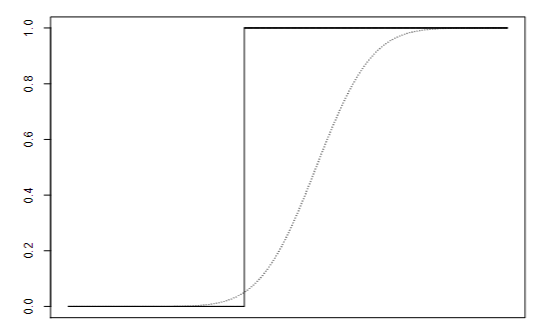
\includegraphics{figures/power_fuction.png}
    \caption[]{效应函数}
\end{figure}

然而这一般只出现在某些很简单的情况(例如$\Uniform(0,1) \vs \Uniform(2,3)$)才有可能发生。通常情况是如果要降低 $\alpha$,则需要扩大接受域的范围,而这会减小拒绝域的范围,导致 $\beta$ 增大;如果要减小 $\beta$,则需要扩大拒绝域的范围,而这会减小接受域的范围,导致 $\alpha$ 增大。

Neyman-Pearson范式将原假设与对立假设置于不平等的地位:显著性水平$\alpha$将被优先考虑,保证其低于某个固定值(例如0.1,0.05或0.01),这称之为保护原假设;接下来再尝试构造一个效应函数 $\pi(\theta;W),\ \theta \in \Theta_A$尽量小的检验。这称之为(显著性) $\alpha$级别的检验。

在显著性为 $\alpha$的前提下,什么是最好的检验?如何比较两个检验哪个更好?

\begin{definition}[一致最大功效检验]
    若在所有显著性为 $\alpha$的检验中,存在一种检验,在任意 $\theta \in \Theta_A$中,其效应函数都大于等于其他检验,则称这种检验为\textbf{一致最大功效检验}(uniformly most powerful tests, UMP)。
\end{definition}

\subsection{p值}

继续考虑例题\ref{ex:coins}的情景。$X \sim \Binomial(10, p)$,
\[ H_0: p=0.5 \vs H_A : p = 0.7 \]
在这种情况中,观测值$X$越大,对 $H_A$的支持越强,即拒绝域应包含$X$中的较大值。能够越强力地支持$H_A$的观测值称\textbf{越极端}的。若将拒绝域设为 $W=\{ 7,8,9,10 \}$,则显著性水平为
\[ \alpha = \P(X \in W|p=0.5) = 0.18 \]
效应为
\[ 1-\beta= \P(X \in W|p=0.7)=0.65\]

\begin{definition}
    
\end{definition}

\subsection{统计显著性}

\section{一些标准检验}

\section{然似比检验}

\begin{definition}[似然比]
    设样本 $x=(X_1,\cdots X_n)$的联合概率密度(质量)函数为 $f \in \Theta=\{ f_0, f_A \}$,检验为:
    \[ H_0: f = f_0 \vs H_A: f=f_A \]
    则称下式为检验\textbf{似然比}(likehood ratio)。
    \[ \frac{f_0(x)}{f_A(x)} \]
\end{definition}

这也是体现数据极端性的一种定义,当似然比越小,则数据越极端。为何不用 $f_0(x)-f_A(x)$体现?$f_0(x), f_A(x)$往往很小,即使两者比例差很大时,其差值也很小,不能体现其意义。

\begin{theorem}[Neyman-Pearson 引理]

\end{theorem}


\begin{problemset}[错题记录]
    \item (茆7.1.1)
    \item
\end{problemset}

\chapter{区间估计}

\section{区间估计的概念}

\section{枢轴变量法}

\subsection{正态总体参数}

\subsection{非正态总体参数}

\section{Fisher的信仰推断法}

\section{容忍区间于容忍限}

\begin{problemset}[错题记录]
    \item (茆6.6.11)
    \item (茆6.6.13)
    \item (茆6.6.15-18)
    \item (茆6.6.20-24)
\end{problemset}
\chapter{抽样分布}

\section{统计量的极限分布}





\section{充分统计量}

若样本数据量大,可能难以解释。试验者希望提取样本值的一些关键特征以概括样本中的信息。这类数据简化(缩减)在计算统计学中通常以样本函数的形式实现,例如,样本均值、样本方差、最大观测值和最小观测值就是四个概括样本关键特征的统计量。

任意一个统计量$T(X)$都定义了一种数据简化方式。如果试验者只观测统计量$T(x)$而非整个样本$x$,则他必将满足$T(x) = T(y)$的$x$和$y$视作两个相同的样本,尽管事实可能并非如此。不同的统计量对数据中的信息划分有不同的方法。

依据某统计量简化样本数据可以看成样本空间$\mathcal{X}$上的一个划分。设
\[ \mathcal{T}=\{t|\exists x \in \mathcal{X}, \text{s.t.} \quad  t=T(x) \} \]
为$\mathcal{X}$在$T(x)$下的象。则
\[ A_t=\{x|T(x)=t, t \in \mathcal{T}\} \]
为$\mathcal{X}$若干划分。

原始数据包含了所有信息,规律或随机部分。若进行转化,则将丢失信息,可能有用,也可能无用。其中界限由假设的统计模型判断。转化后的可能结果:
\begin{enumerate}
	\item 留下部分有用信息:完备统计量
	\item 留下所有有用信息:充分统计量
	\item 不留下有用信息:辅助统计量
\end{enumerate}

\begin{example}
	设$X_1,\dots,X_n \thicksim Binomial(p) \quad \text{i.i.d.} $,设$T(X)=\sum X_i$。
	若$T=t$已知,则实验结果与$p$无关,由于:
	$$P(X|T)=\frac{P(X)}{P(T)}=\frac{p^t(1-p)^{n-t}}{\binom{n}{t} p^t(1-p)^{n-t}}=\frac{1}{\binom{n}{t}}$$
\end{example}

\begin{remark}
	$T \thicksim Binomial(n,p)$与$p$有关,而$X|T$与参数无关。即原始数据经$T$转化后的$T(X)$,仍包含所有关于参数的信息;而余下的$X|T$不再包含参数信息。
\end{remark}

\begin{definition}[充分统计量]
	假设样本$X$,满足分布$P(\theta)$,若统计量$S(X)$,$P(X|S)$与$\theta$无关,则称$S(X)$为关于$\theta$的充分统计量。
\end{definition}

\begin{remark}
	充分统计量的判断与统计模型有关,模型不当可能导致充分统计量实际不“充分”。
\end{remark}

\begin{theorem}[分解定理]
	$S(X)$为关于$\theta$的充分统计量的充要条件为:
	$$\exists g(),h() \text{s.t.} f(X|\theta)=g(S(X),\theta)h(X)$$
\end{theorem}

\begin{remark}
	直观理解:$P(X)=P(S)P(X|S)$
\end{remark}

\begin{proof}
	对于离散情况:\\
	充分:
	$$P(S=s)=\sum_{S(x)=s}P(X=x)=g(s,\theta)\sum_{S(x)=s}h(x)$$
	$$P(X=x|S=s)=\frac{P(X=x)}{P(S=s)}=\frac{h(x)}{\sum_{S(x)=s}h(x)}$$
	与$\theta$无关。\\
	必要:\\
	令$$g(s,\theta)=P(T=s|\theta),h(x)=P(X=x|S=s)$$即可
\end{proof}

\begin{theorem}
	若$S(X)$为关于$\theta$的充分统计量,则$\theta$的极大然似估计可表示为$S$的函数。
\end{theorem}

\begin{proof}
	然似函数为$g(S,\theta)h(X)$。由于$h(X)$为定值,故只需求$g(S,\theta)$的极值情况,故$\theta$的取值可由$S$的函数表示。
\end{proof}

为使数据尽可能精简,摈弃无用信息,定义极小充分统计量。

\begin{definition}[极小充分统计量]
	若统计量$M$满足
	$$\forall S, \exists h  \quad \text{s.t.} \quad
	 M=h(S) $$
	则其为关于$\theta$的充分统计量
\end{definition}

\section{完全统计量}



\chapter{线性模型}

\section{回归分析}

\section{最小二乘法}

\section{方差分析}


\appendix
\chapter{附录}

\section{指数族}

指数族(Exponential Families)是数理统计中非常重要的一个分布族

\begin{definition}[指数族]
	对于参数分布族 $\{ P_\theta: \theta \in \Theta \}$,若存在分布族的充分统计量$T(x)$,参数空间上的向量值函数 $\eta(\theta)$,实值函数 $B(\theta)$和非负可测函数 $h(x)$,使得分布族的密度函数看表示为:
	\[ f_{\theta}(x) = h(x) \exp\{\eta(\theta)^{\top}T(x)-B(\theta)\}  \]
    则称分布族$\{ P_\theta: \theta \in \Theta \}$为\textbf{指数族}(Exponential Families)。其中$B(\theta)$称为\textbf{势函数},可写为:
    \[ B(\theta)=\ln \int_{\Omega}h(x) \exp\{\eta(\theta)^{\top}T(x)\} \d x  \]
\end{definition}

由指数族密度函数的性质可以立刻得到,指数族的支撑集仅与 $h(x)$ 相关,与未知参数 $\theta$ 无关。若分布族的支撑集与未知参数相关,如 $[0,\theta]$ 上的均匀分布族,则该分布族一定不是指数族。

常见的指数族有:正态分布、卡方分布、二项分布、多项分布、Poisson分布、Pascal分布、beta分布、gamma分布、对数正态分布等;常见的非指数族有:均匀分布、带有位置参数(location parameters)的指数分布、极值分布、Weibull分布、超几何分布、Cauchy分布、Laplace分布等。

\section{多元正态分布}

\end{document}